%%%%%%%%%%%%%%%%%%%%%%%%%%%%%%%%%%%%%%%%%%%%%%%%%%%%%%%%%%%%%%%%%%%%%%%%%%%%%
\chapter{Implementation}\label{chap:impl}
%%%%%%%%%%%%%%%%%%%%%%%%%%%%%%%%%%%%%%%%%%%%%%%%%%%%%%%%%%%%%%%%%%%%%%%%%%%%%
\chapterstart

This Chapter provides infromation about Solidity, the programming language used for the EtherLotto Smart Contract, the frontend implementation as well as the tools and frameworks used during development.


%%%%%%%%%%%%%%%%%%%%%%%%%%%%%%%%%%%%%%%%%%%%%%%%%%%%%%%%%%%%%%%%%%%%%%%%%%%%%
\section{ Smart Contract with Solidity}\label{sec:solidity}
%%%%%%%%%%%%%%%%%%%%%%%%%%%%%%%%%%%%%%%%%%%%%%%%%%%%%%%%%%%%%%%%%%%%%%%%%%%%%

The implementation of the Ethereum Smart Contract can be done in various programming languages. However, the most common and well documented one is Solidity and was therefore chosen for this project work.

Solidity is a contract-oriented, high-level language for implementing smart contracts. It was influenced by C++, Python and JavaScript and is designed to target the \ac{EVM}.

Solidity is statically typed, supports inheritance, libraries and complex user-defined types among other features.


A simple Example in Solidity:
\begin{lstlisting}[language=Solidity]
pragma solidity ^0.4.0; // defines the solidity version

contract SimpleStorage { // = collection of functions and data
    uint storedData; // unsigned integer variable

    // public setter
    function set(uint x) public {
        storedData = x;
    }

    // public getter
    function get() public constant returns (uint) {
        return storedData;
    }
}
\end{lstlisting}

\begin{flushright}
Source: \citetitle{solidity}
\end{flushright}

%%%%%%%%%%%%%%%%%%%%%%%%%%%%%%%%%%%%%%%%%%%%%%%%%%%%%%%%%%%%%%%%%%%%%%%%%%%%%
\subsection{Solidity Remix \ac{IDE}}\label{sec:ide}
%%%%%%%%%%%%%%%%%%%%%%%%%%%%%%%%%%%%%%%%%%%%%%%%%%%%%%%%%%%%%%%%%%%%%%%%%%%%%

For ease of use during development of the EtherLotto Smart Contract, the Remix \ac{IDE} for Solidity was used. The Remix \ac{IDE} is a Web \ac{IDE} designed for Solidity \ac{DApp} developers. It offers syntax highlighting, static analysis and debugging tools via a JavaScript \ac{EVM} running in the browser without any installation required by the developer.

\begin{figure}[h]
  \centering
  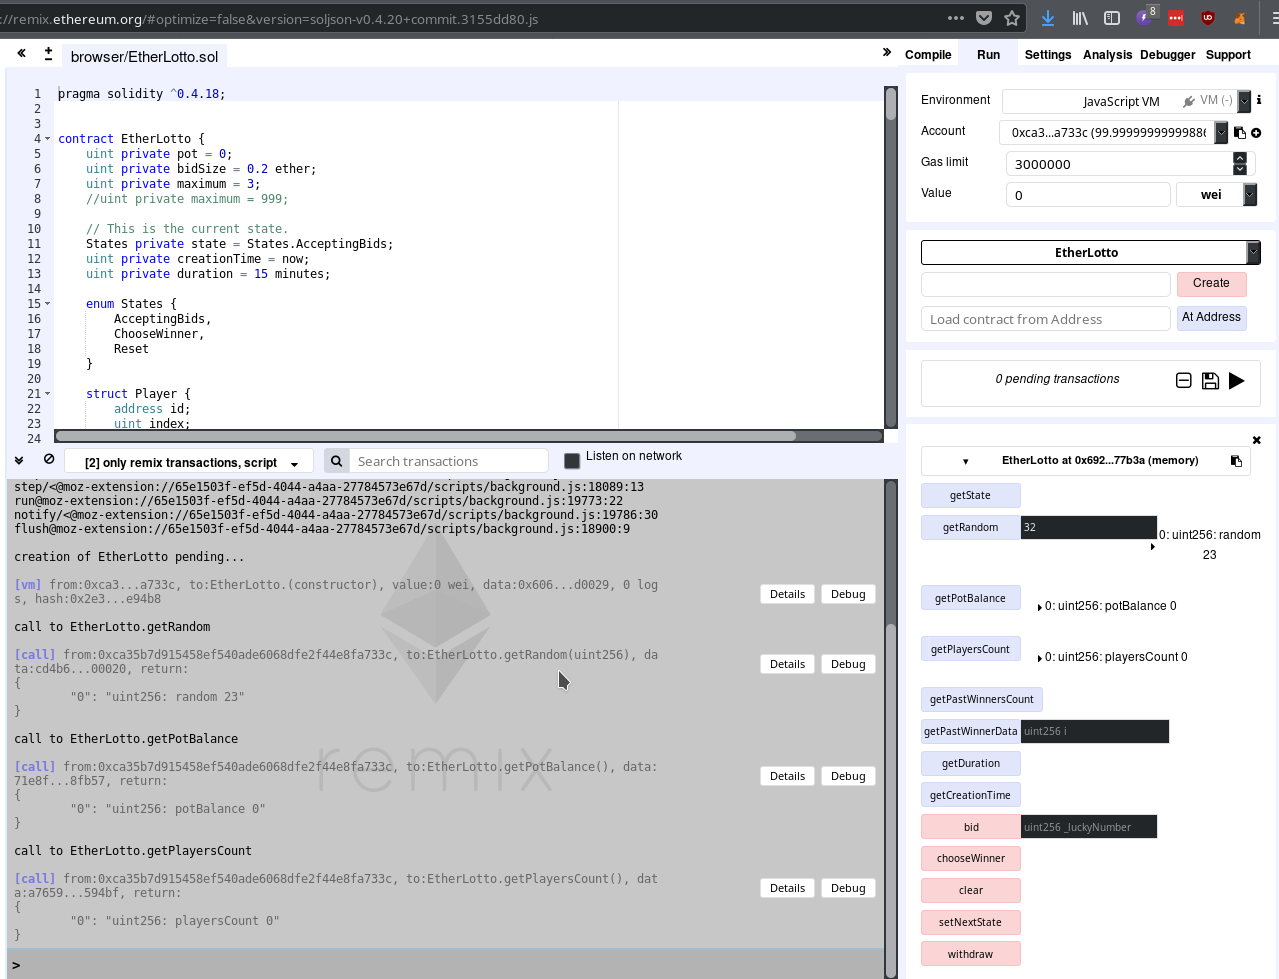
\includegraphics[keepaspectratio,width=0.95\textwidth]{images/remix}
  \caption[Remix IDE]{Remix IDE. Contract is running in a JavaScript \ac{EVM}, all functions can be called and debugged.}
  \label{fig:remix}
\end{figure}


%%%%%%%%%%%%%%%%%%%%%%%%%%%%%%%%%%%%%%%%%%%%%%%%%%%%%%%%%%%%%%%%%%%%%%%%%%%%%
\subsection{Lottery States}\label{sec:states}
%%%%%%%%%%%%%%%%%%%%%%%%%%%%%%%%%%%%%%%%%%%%%%%%%%%%%%%%%%%%%%%%%%%%%%%%%%%%%

A lottery usually goes through several states. From the start of the lottery, where bids are accepted, to the drawing of the winner and payout of the sum won.

Therefore in Solidity the following states where defined using Enums:

\begin{lstlisting}[language=Solidity]
// This is the current state.
States private state = States.AcceptingBids;

    enum States {
    AcceptingBids,
    ChooseWinner,
    Reset
}
\end{lstlisting}

An Enum is a way in Solidity to create a user-defined type. They are explicitly convertible to and from all integer types but implicit conversion is not allowed. The explicit conversions check the value ranges at runtime and a failure causes an exception. Enums needs at least one member.

Based on these Enums and the variable state, it is possible to determine the current state of the Lottery and make only specific function available.

To transition between these states, custom function modifiers can be created. These modifiers not only handle the transition between states, but also restrict access to functions not allowed in the current state.

\begin{lstlisting}[language=Solidity]
// modifier to restrict access
modifier atState(States _state) {
    // throws exception if condition not met
    require(state == _state);
    
    // code from the function being modified is inserted here
    _;
}

// function so set the next state
function nextState() internal {
    // increment state by 1
    state = States(uint(state) + 1);
}

// modifier to trasition to the next state after function execution
modifier transitionNext() {
    // code from the function being modified is inserted here
    _;
    
    nextState();
}

// transistion modifier with time condition
modifier timedTransitions() {
    if (state == States.AcceptingBids && now >= creationTime + duration)
        nextState();
        
    // code from the function being modified is inserted here
    _;
}
\end{lstlisting}

A modifier can then simply be added to a function declaration.

\begin{lstlisting}[language=Solidity]
// only possible to call when state = Reset
function clear() public atState(States.Reset) {
    playerIndex = 0;
    players.length = 0;
    winnerIndex = 0;
    winners.length = 0;
    state = States.AcceptingBids;
    creationTime = now;
}
\end{lstlisting}


%%%%%%%%%%%%%%%%%%%%%%%%%%%%%%%%%%%%%%%%%%%%%%%%%%%%%%%%%%%%%%%%%%%%%%%%%%%%%
\subsection{Player and Winner data struct}\label{sec:structs}
%%%%%%%%%%%%%%%%%%%%%%%%%%%%%%%%%%%%%%%%%%%%%%%%%%%%%%%%%%%%%%%%%%%%%%%%%%%%%

To save players, determine winners and in turn also save them, custom data types where necessary.

In Solidity this can be realized via Structs and is somewhat similar to Structs in C/C++.

\begin{lstlisting}[language=Solidity]
struct Player {
    address id; // Ethereum address
    uint index; // player index
    uint luckyNumber; // number the player bet on
}

// array of players
Player[] private players;
uint private playerIndex = 0;

// array of winners in the current round
Player[] private winners;
uint private winnerIndex = 0;


struct PastWinner {
    Player player; // the player who won
    uint amount; // the amount won
    uint winningTime; // the time the player won
}

// array of all-time winners
PastWinner[] private pastWinners;
\end{lstlisting}


%%%%%%%%%%%%%%%%%%%%%%%%%%%%%%%%%%%%%%%%%%%%%%%%%%%%%%%%%%%%%%%%%%%%%%%%%%%%%
\subsection{Events}\label{sec:events}
%%%%%%%%%%%%%%%%%%%%%%%%%%%%%%%%%%%%%%%%%%%%%%%%%%%%%%%%%%%%%%%%%%%%%%%%%%%%%

Events allow the convenient usage of the \ac{EVM} logging facilities, which in turn can be used to trigger JavaScript callbacks in the user interface of a \ac{DApp}, which listen for these events.

However, in this Project Work Events are simply used to log relevent information.


\begin{lstlisting}[language=Solidity]
// event declaration
event NewBidRecieved(address id, uint index, uint amount, uint luckyNumber);
event CalculatedNewRandom(uint random);
event StateChanged(States state);


function nextState() internal {
    state = States(uint(state) + 1);
    // trigger event
    StateChanged(state);
}
\end{lstlisting}

%%%%%%%%%%%%%%%%%%%%%%%%%%%%%%%%%%%%%%%%%%%%%%%%%%%%%%%%%%%%%%%%%%%%%%%%%%%%%
\subsection{Placing a bid}\label{sec:bet}
%%%%%%%%%%%%%%%%%%%%%%%%%%%%%%%%%%%%%%%%%%%%%%%%%%%%%%%%%%%%%%%%%%%%%%%%%%%%%

The following function can be called to place a new bid:

\begin{lstlisting}[language=Solidity]
function bid(uint _luckyNumber) public payable timedTransitions atState(States.AcceptingBids) {
    // check correct amount sent
    require(msg.value == bidSize);
    // check numbe rin range
    require(_luckyNumber != 0 && _luckyNumber < (maximum + 1)); 

    // trigger event
    NewBidRecieved(msg.sender, playerIndex, msg.value, _luckyNumber);

    // add amount sent to pot size
    pot += msg.value;
    // add new player to array
    insertPlayer(Player(msg.sender, playerIndex, _luckyNumber));
}
\end{lstlisting}

The modifier payable indicates that this function can recieve ether, timedTransitions and atState are explained in Section~\ref{sec:states}.


%%%%%%%%%%%%%%%%%%%%%%%%%%%%%%%%%%%%%%%%%%%%%%%%%%%%%%%%%%%%%%%%%%%%%%%%%%%%%
\subsection{Random Generation}\label{sec:random}
%%%%%%%%%%%%%%%%%%%%%%%%%%%%%%%%%%%%%%%%%%%%%%%%%%%%%%%%%%%%%%%%%%%%%%%%%%%%%

A random Generation in a deterministic Blockchain like the one Ethereum uses is impossible. Therefore the random number is calculated from the bblockhash of the next block generated after the state of the changed to ChooseWinner. In this state no additional bids are accepted. This method of calculating a pseudo-random number is potentially manipulateable, because a miner controlling about 50\% the Ethereum hash calculation could influence the next blockhash by invalidating the calculated block if he chooses. Since this magnitude of manipulation is extremely resource heavy, it is no feasable to use it for such small amounts of Ether used in this demo /ac{DApp}.

Function to get the pseudo-random number:
\begin{lstlisting}[language=Solidity]
function getRandom(uint _maximum) public view returns (uint random) {
    return uint(block.blockhash(block.number-1)) % _maximum + 1;
}
\end{lstlisting}

%%%%%%%%%%%%%%%%%%%%%%%%%%%%%%%%%%%%%%%%%%%%%%%%%%%%%%%%%%%%%%%%%%%%%%%%%%%%%
\subsection{Choosing a Winner}\label{sec:winner}
%%%%%%%%%%%%%%%%%%%%%%%%%%%%%%%%%%%%%%%%%%%%%%%%%%%%%%%%%%%%%%%%%%%%%%%%%%%%%

The following snippet chooses all winners for a lottery round and lets them withdraw their share of the pot.

\begin{lstlisting}[language=Solidity]
function chooseWinner() public timedTransitions atState(States.ChooseWinner) {
    // get random number
    uint winningNumber = getRandom(maximum);

    // trigger event
    CalculatedNewRandom(winningNumber);

    // get winners and insert them into winners array
    getWinners(winningNumber);

    if (winners.length > 0) {
        // set the amount each winner can withdraw
        setPendingWithdrawals();
    }

    // transition to Reset state
    nextState();
    clear();
}

function getWinners(uint winningNumber) internal {
    for (uint i = 0; i < playerIndex; i++) {
        if (players[i].luckyNumber == winningNumber) {
            insertWinner(players[i]);
        }
    }
}

function setPendingWithdrawals() internal {
    uint potPerWinner = pot / winners.length;
    pot = 0;

    for (uint i = 0; i < winnerIndex; i++) {
        pendingWithdrawals[winners[i].id] += potPerWinner;
        pastWinners.push(PastWinner(winners[i], potPerWinner, now));
    }
}
\end{lstlisting}


%%%%%%%%%%%%%%%%%%%%%%%%%%%%%%%%%%%%%%%%%%%%%%%%%%%%%%%%%%%%%%%%%%%%%%%%%%%%%
\subsection{Withdrawing Ether}\label{sec:withdraw}
%%%%%%%%%%%%%%%%%%%%%%%%%%%%%%%%%%%%%%%%%%%%%%%%%%%%%%%%%%%%%%%%%%%%%%%%%%%%%

The recommended method of sending funds after an effect is using the withdrawal pattern. Although the most intuitive method of sending Ether, as a result of an effect, is a direct send call, this is not recommended as it introduces a potential security risk.

\begin{lstlisting}[language=Solidity]
function withdraw() public {
    uint amount = pendingWithdrawals[msg.sender];
    // Remember to zero the pending refund before
    // sending to prevent re-entrancy attacks
    pendingWithdrawals[msg.sender] = 0;
    msg.sender.transfer(amount);
}
\end{lstlisting}

\newpage

%%%%%%%%%%%%%%%%%%%%%%%%%%%%%%%%%%%%%%%%%%%%%%%%%%%%%%%%%%%%%%%%%%%%%%%%%%%%%
\section{Frontend with Truffle Framework}\label{sec:truffle}
%%%%%%%%%%%%%%%%%%%%%%%%%%%%%%%%%%%%%%%%%%%%%%%%%%%%%%%%%%%%%%%%%%%%%%%%%%%%%

Truffle is a JavaScript development framework for Ethereum. It provides built-in Smart Contract compilation, linking, deployment and binary management via an interactive console called the truffle environment or deployment scripts. In addition to that it also provides an environment for automated contract testing using either Solidity or JavaScript.

More information on truffle and all its features can be found in the \citetitle{truffleDocs} and \citetitle{truffleTutorial}.

\begin{flushright}
Source: \citetitle{truffle}
\end{flushright}

Using truffle it is relatively easy to build a frontend for any type of interaction with a Smart Contract deployed on the Blockchain. Since the Smart Contract is also compiled and deployed with truffle, there are no extra steps necessary to give the frontend implementation the necessary artifact files. Artifact files provide the interface to communicate with a deployed Smart Contract and its functions.

All that is left to do before communcation is possible, is to spcify a Provider. The Provider holds information on which Ethereum network to use and how to communicate with it without running a full Ethereum node which is usually needed to make transaction on the Ethereum Blockchain. At the time of writing, the easiest way to provide this is a broweser addon called /citetitle{metamask}. /citetitle{metamask} includes a secure identity vault, providing a user interface to manage your identities on different sites and sign blockchain transactions.

The following shows an Example of how to call a Smart Contract function with JavaScript using Promises for safe execution and error handling.
\begin{lstlisting}
withdraw = () => {
    this.EtherLotto
        .deployed()
        .then(instance => {
        return instance.withdraw({from: this.account});
    }).then(() => {
        console.log('Withdraw complete!');
        this.getBalance();
    }).catch(function(e) {
        console.log(e);
        this.setStatus('Error withdrawing coins; see log.');
    });
};
\end{lstlisting}

\newpage
%%%%%%%%%%%%%%%%%%%%%%%%%%%%%%%%%%%%%%%%%%%%%%%%%%%%%%%%%%%%%%%%%%%%%%%%%%%%%
\section{User Interface}\label{sec:ui}
%%%%%%%%%%%%%%%%%%%%%%%%%%%%%%%%%%%%%%%%%%%%%%%%%%%%%%%%%%%%%%%%%%%%%%%%%%%%%

The User Interface for this demo \ac{DApp} was kept as simple as possible providing a Material Design approach using \citetitle{angularMaterial}.

\begin{figure}[h]
  \centering
  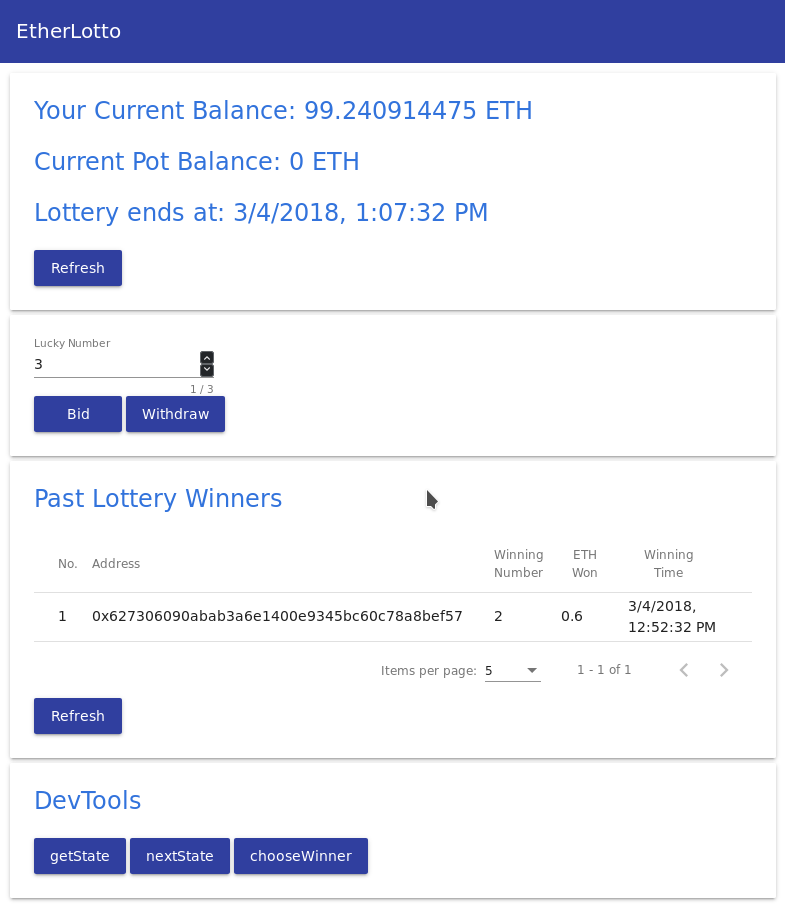
\includegraphics[keepaspectratio,width=0.95\textwidth]{images/ui}
  \caption[EtherLotto UI]{EtherLotto Material Design User Interface}
  \label{fig:ui}
\end{figure}

\newpage
%%%%%%%%%%%%%%%%%%%%%%%%%%%%%%%%%%%%%%%%%%%%%%%%%%%%%%%%%%%%%%%%%%%%%%%%%%%%%
\section{Tests with Truffle Framework}\label{sec:truffleTest}
%%%%%%%%%%%%%%%%%%%%%%%%%%%%%%%%%%%%%%%%%%%%%%%%%%%%%%%%%%%%%%%%%%%%%%%%%%%%%

As already mentioned in Section \nameref{sec:truffle}, truffle comes standard with automated contract testing framework using either Solidity or JavaScript.

Truffle provides a clean room environment when running test files. When running tests against \citetitle{ganache}\footnote{Ganache provides a local Blockchain to run tests, execute commands and inspect states while controllin ghow the chain operates} or Truffle Develop, Truffle will use advanced snapshotting features to ensure test files don't share their state with each other.

%%%%%%%%%%%%%%%%%%%%%%%%%%%%%%%%%%%%%%%%%%%%%%%%%%%%%%%%%%%%%%%%%%%%%%%%%%%%%
\subsection{Solidity Tests}\label{sec:solTest}
%%%%%%%%%%%%%%%%%%%%%%%%%%%%%%%%%%%%%%%%%%%%%%%%%%%%%%%%%%%%%%%%%%%%%%%%%%%%%

Solidity tests are included as a seperate test suite per test-contract during execution, have direct access to deployed contracts and can potentially import andy contract dependency. In addition to that, the assertion library can be changed at any time and tests can be run against any Ethereum client. More information can be found in the \citetitle{truffleDocs}.

Example of a simple Solidity test:
\begin{lstlisting}[language=Solidity]
pragma solidity ^0.4.2;

import "truffle/Assert.sol";
import "truffle/DeployedAddresses.sol";
import "../contracts/EtherLotto.sol";


contract TestEtherLotto {
    // Truffle will send the TestContract one Ether after deploying the contract.
    uint public initialBalance = 1 ether;

    function testInitialPotBalance() public {
        EtherLotto etherLotto = EtherLotto(DeployedAddresses.EtherLotto());

        uint expextedPot = 0;

        Assert.equal(etherLotto.getPotBalance(), expextedPot, "Initial Pot Balance should always be 0");
    }
}
\end{lstlisting}


%%%%%%%%%%%%%%%%%%%%%%%%%%%%%%%%%%%%%%%%%%%%%%%%%%%%%%%%%%%%%%%%%%%%%%%%%%%%%
\subsection{Javascript Tests}\label{sec:jsTest}
%%%%%%%%%%%%%%%%%%%%%%%%%%%%%%%%%%%%%%%%%%%%%%%%%%%%%%%%%%%%%%%%%%%%%%%%%%%%%

Truffle uses the \citetitle{mocha} unit testing framework and therefore works mostly similiar to a standard Mocha test. The only exception is that instead of \lstinline{describe()}, the truffle specific \lstinline{contract()} function is used. This enables all clean room features described in Section \nameref{sec:truffleTest}. 

This means that:
\begin{itemize}
    \item Before each \lstinline{contract()} function is run, all contracts are re-deployed to provide a clean state.
    \item The \lstinline{contract()} function provides a list of test accounts made available by the Ethereum client.
\end{itemize}

The following code snippet shows a JavaScript test to validate the pot balance after one recieved bid using the NewBidRecieved Event implemented in the EtherLotto Smart Contract.
\begin{lstlisting}[language=JavaScript]
var EtherLotto = artifacts.require("EtherLotto");

contract('EtherLotto', function(accounts) {
  it("test contract deployed", function() {
    return EtherLotto.deployed().then(function(instance) {
      assert(instance != undefined, "contract is not correctly deployed");
    });
  });

  it("test pot balance after one bid", function() {
    var etherLotto;
    var expectedBid = 200000000000000000;
    var expectedLuckyNumber = 1;
    var expectedIndex = 0;

    return EtherLotto.deployed().then(function(instance) {
      etherLotto = instance;
      // execute bid function
      return etherLotto.bid(expectedLuckyNumber, {from: accounts[0], value: expectedBid});
    }).then(function(result) {

      var recievedBidValue;
      var recievedPlayerAddress;
      var recievedLuckyNumber;
      var recievedIndex;

      // parse result for NewBidRecieved-Event
      for (var i = 0; i < result.logs.length; i++) {
        var log = result.logs[i];

        if (log.event == "NewBidRecieved") {
          recievedPlayerAddress = log.args.id;
          recievedBidValue = log.args.amount.toNumber();
          recievedLuckyNumber = log.args.luckyNumber.toNumber();
          recievedIndex = log.args.index.toNumber();
        }
      }

      assert.equal(recievedPlayerAddress, accounts[0], "address from event and sender address need to match");
      assert.equal(recievedBidValue, expectedBid, "bid value from event and sent bid have to match");
      assert.equal(recievedIndex, expectedIndex, "index should match");
      assert.equal(recievedLuckyNumber, expectedLuckyNumber, "lucky Number should match");

      return etherLotto.getPotBalance();
    }).then(function(balance) {
      // check pot balance
      assert.equal(balance.toNumber(), expectedBid, "wrong value in potBalance, bid went wrong");
    });
  });
});
\end{lstlisting}

\newpage
%%%%%%%%%%%%%%%%%%%%%%%%%%%%%%%%%%%%%%%%%%%%%%%%%%%%%%%%%%%%%%%%%%%%%%%%%%%%%
\subsection{Executing Tests}\label{sec:execTests}
%%%%%%%%%%%%%%%%%%%%%%%%%%%%%%%%%%%%%%%%%%%%%%%%%%%%%%%%%%%%%%%%%%%%%%%%%%%%%

The easiest way to run Truffle tests is with the built-in Ethereum Client and interactive shell. To start it simply run the following command in the root directory of the truffle project.
\begin{lstlisting}[language=bash]
$ truffle develop
\end{lstlisting}
This will start a local Ethereum Blockchain and generate accounts with some Ether in their wallet.

Using the interactive shell, the tests can now be run directly.
\begin{lstlisting}[language=bash]
truffle(develop)> test
Using network 'develop'.

Compiling ./contracts/EtherLotto.sol...
Compiling ./test/TestEtherLotto.sol...
Compiling truffle/Assert.sol...
Compiling truffle/DeployedAddresses.sol...


  TestEtherLotto
     testInitialPotBalance (71ms)

  Contract: EtherLotto
     test contract deployed
     test pot balance after one bid (55ms)

  Contract: EtherLotto
     test a full lottery (577ms)


  4 passing (1s)
\end{lstlisting}




\chapterend

